\documentclass[tikz,border=8pt]{standalone}
\usepackage[T1]{fontenc}
\usepackage[sfdefault]{FiraSans}
\usepackage{tikz}
\usetikzlibrary{arrows.meta,positioning,calc,decorations.pathreplacing}
\definecolor{navy}{HTML}{003C6C}
\definecolor{navydeep}{HTML}{06294A}
\definecolor{ink}{HTML}{18293B}
\definecolor{muted}{HTML}{5B6B7C}
\definecolor{gold}{HTML}{FDC700}
\definecolor{amber}{HTML}{C98A00}
\definecolor{teal}{HTML}{0E7C9C}
\definecolor{coral}{HTML}{E4572E}
\definecolor{hairline}{HTML}{D9E1E9}
\definecolor{skyfill}{HTML}{E7F0F7}

\begin{document}
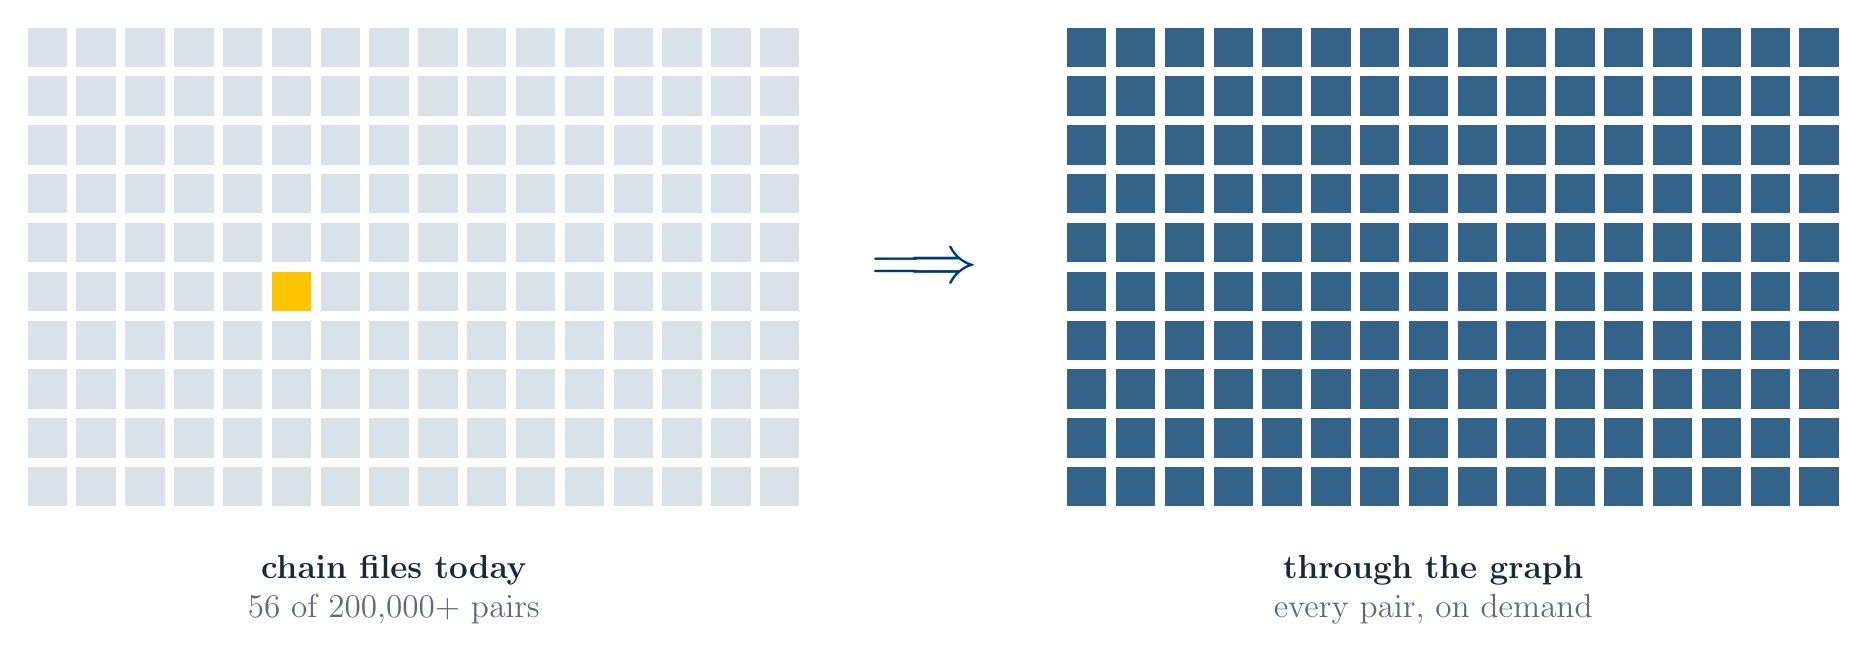
\begin{tikzpicture}
  \foreach \x in {0,...,15}
    \foreach \y in {0,...,9}
      {\fill[hairline] (\x*0.62,\y*0.62) rectangle +(0.5,0.5);}
  \fill[gold] (5*0.62,4*0.62) rectangle +(0.5,0.5);
  \node[anchor=north, font=\large, text=muted, align=center]
    at (4.65,-0.5) {\textbf{\color{ink}chain files today}\\ 56 of 200{,}000+ pairs};
  \node[font=\Huge, text=navy] at (11.4,3.0) {$\Longrightarrow$};
  \begin{scope}[shift={(13.2,0)}]
    \foreach \x in {0,...,15}
      \foreach \y in {0,...,9}
        {\fill[navy!80] (\x*0.62,\y*0.62) rectangle +(0.5,0.5);}
    \node[anchor=north, font=\large, text=muted, align=center]
      at (4.65,-0.5) {\textbf{\color{ink}through the graph}\\ every pair, on demand};
  \end{scope}
\end{tikzpicture}
\end{document}
